\documentclass{article}
\usepackage{hyperref}
\usepackage{amsmath}
\usepackage{amssymb}
\usepackage{pgfplots}
\usepackage{float}
\usepackage{todonotes}
\usepackage{tikz}
\usepackage[shortlabels]{enumitem}

\renewcommand{\Re}{\mathbb{R}}
\newcommand{\Li}{\mathcal{L}}
\newcommand{\Ex}{\mathbb{E}}
\renewcommand{\Pr}{\mathbb{P}}
\newcommand{\Hy}{\mathcal{H}}
\newcommand{\sign}{\text{sign}}
\newcommand{\error}{\text{error}}

\newcommand\bigO[1]{
    \ensuremath{\mathcal{O}\left(#1\right)}
    }

\newcommand{\sigmoidPlot}{
    
    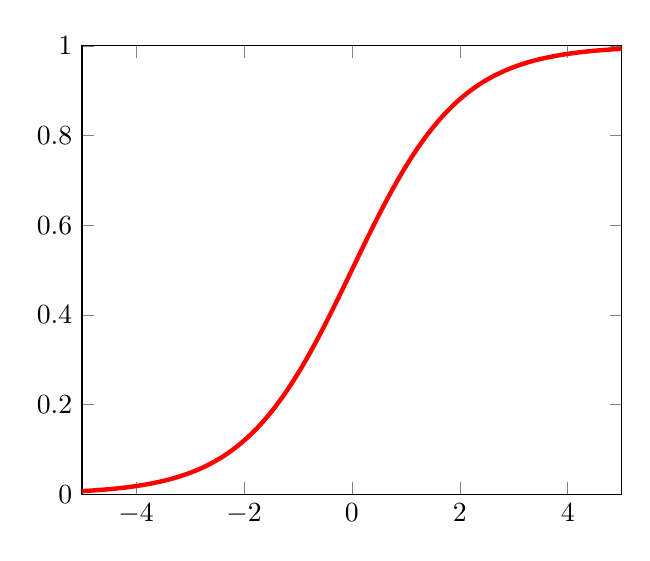
\begin{tikzpicture}
        \begin{axis}[xmin=-5, xmax=5, ymin=0, ymax=1, samples=150]
        \addplot[red, ultra thick] {1/(1+exp(-x))};
        \end{axis}
    \end{tikzpicture}
    
    }

\usetikzlibrary{positioning, calc}
\usetikzlibrary{arrows.meta}

\tikzstyle{circlebox}=[circle,thick,draw=black!75,minimum size=8mm]
\tikzstyle{inputnode}=[circlebox, draw=blue!75]
\tikzstyle{hiddennode}=[circlebox, draw=orange!75]
\tikzstyle{outputnode}=[circlebox, draw=orange!75]
\tikzstyle{simplebox}=[rectangle,thick,draw=black!75,
fill=black!20,minimum size=4mm]
\tikzstyle{textbox}=[rectangle,thick,minimum size=4mm,draw=black!0,
fill=black!0]
\tikzstyle{halfvdistance}=[yshift=-0.7cm]
\tikzstyle{abovebetween}=[xshift=-2.7mm]
\tikzstyle{edgepath} = [-Latex,->,shorten >=1pt,-stealth,semithick, rounded 
corners=5pt]

\def \nodedv {0.735cm}
\def \nodedh {0.65cm}

\tikzset{
    between/.style args={#1 and #2}{
        at = ($(#1)!0.5!(#2)$)
    }
}

\begin{document}
    \section{Subjects}
    \begin{itemize}
        \item What is an evolutionary tree?
        \item Computing an evolutionary tree from distance data.
    \end{itemize}
    
    \section{Notes}
    
    \subsection{Phylogenetic trees}
    There is strong evidence that all life on earth is decended from a single 
    common ancestor. Over the course of at least 3.8 billion years, that life 
    form has changed and split itself into new and independent lineages. The 
    evolutionary relationships among these species is referred to as their 
    phylogeny, phylogenetic reconstruction is concerned with inferring the 
    phylogeny of groups of organisms.
    
    We call these groups \textit{taxa} (or singular taxon), the splitting of 
    lineages is called \textit{speciation} (think of splitting it into 
    different species). Usually speciation happens if one population is split 
    into two that can no longer interbreed (e.g. if a river splits them apart). 
    We can use methods of phylogenetic to contemplate over the tree of life, or 
    simply to inferr the phylogeny of different populations within a species.
    
    In a rooted phylogenetic tree $T$, the root node $r$ corresponds to the 
    last common ancestor of all species in $T$, we then call a path from the 
    root to a leaf an \textit{evolutionary path}. If an equal amount of change 
    occurs on every evolutionary path (i.e. each species have the same amount 
    of ``change'') then the evolutionary change occur in a more-or-less 
    clocklike fashion and we then say that this tree satisfies the 
    \textit{molecular clock hypothesis}, we can then assign a time $t(v)$ to 
    every internal node $v$ in the tree and a length of $t(v)-t(w)$ to an edge 
    $(v,w)$ in the tree.
    
    Every extant (still alive) species corresponds to time $0$, and a 
    speciation event (internal node $v$) occured in the tree $t(v)$ time ago. 
    We then have that the length of an edge represents the amount of time that 
    lies between two speciation events.
    
    Furthermore, the last common ancestor (root) lived $t(r)$ and all 
    evolutionary paths have the same length $t(r)$ where the length of a path 
    is the sum of the lengths of all edges along the path.
    
    Once the \textit{molecular clock hypotheses} was widely accepted, but has 
    since been disproven so now time instead refers to the expected amount of 
    evolution.
    
    \subsubsection{Distance methods}
    Distance methods construct a phylogenetic tree from a distance matrix that 
    contains the evolutionary distances between all pairs of taxa (groups of 
    organisms). If we ignore edge weights, we speak of the topology (shape) of 
    a tree, and it turns out that we have methods that \textit{provably} find 
    the correct tree if the distance matrix is ultrametric, and some that works 
    if the distance matrix is additive. However the data we can record is 
    usually approximation of the true (additive) data, and thus we can't rely 
    on the distance matrix being additive. However, it turns out that the 
    methods can still find the correct \textit{topology} of the tree under 
    certain criteria.
    
    If we just have the topology, then we must assign weights to the edges of 
    the tree that best fit the data, which can be done with the least squares 
    methods.
    
    \subsubsection{Basic definitions}
    Phylogenies are usually represented as binary trees, because generially 
    speciation happens when one lineage splits into two independent lineages. 
    This is not entirely correct, sometimes horizontal gene-transfer happens 
    and hybrid speciation but it is rare. So for simplicity we just look deal 
    with phylogenetic trees, however let's not insist they have to be binary 
    for the moment:
    
    Let $S=\{s_1,\dots,s_n\}$ be a set of taxa. A phylogenetic tree on $S$ is a 
    triple $T=(V,E,\alpha)$ where:
    \begin{itemize}
        \item $V$ is the set of nodes, $E$ is the set of undirected edges
        \item $(V,E)$ is a an acyclic connected graph, in which there might be 
        a distinguished root node of degree $\geq 2$ and all other internal 
        nodes have a degree $\geq 3$. So either rooted or unrooted. We will 
        denote the set of leaves by $V_L$ and the set of internal nodes by $V_I$
        \item $\alpha$ is a bijection $\alpha: S \rightarrow V_L$ between the 
        set of taxa and the set of leaves
    \end{itemize}
    An edge $(v,w) \in E$ is an external edge if either $v$ or $w$ is a leaf. 
    Otherwise it is an internal edge.
    
    We haven't included edge-weights here, they will be introduced later.
    
    A semimetric on $S$ is a function $d:S\times S\rightarrow \Re_{\geq 0}$ 
    that satisfies, for all $x,y,z \in S$:
    \begin{align*}
        d(x,y) &= 0 \iff x=y\\
        d(x,y) &= d(y,x)
    \end{align*}
    A metric, or distance function on $S$ is a semimetric that satisfies the 
    triangle inequality:
    \begin{equation*}
        d(x,y) \leq d(x,z) + d(z,y)
    \end{equation*}
    A metric $d:S\times S\rightarrow \Re_{\geq 0}$ is called \textit{additive} 
    if it satisfies the \textit{additive inequality}:
    \begin{equation*}
        d(w,x)+d(y,z) \leq \max\{d(x,y)+d(w,z), d(x,z)+d(w,y)\}
    \end{equation*} 
    An \textit{ultrametric} on $S$ is an additive metric that satisfies the 
    \textit{ultrametric inequality}:
    \begin{equation*}
        d(x,y) \leq \max\{d(x,z),d(y,z)\}
    \end{equation*}
    
    A symmetric $n \times n$ matrix $D=(d_{ij})$ satisfying $d_{ii}=0$ and 
    $d_{ij}>0$ for all $i\neq j$ with $i,j \in \{1,\dots,n\}$ is called a 
    dissimilarity matrix. That is, the matrix is symmetric and the diagonal is 
    all $0$s. We will now assume that the input to a phylogenetic 
    reconstruction algorithm is such a dissimilarity matrix. We can now say 
    that the dissimilarity matrix, induces a function $d:S \times S\rightarrow 
    R_{\geq 0}$ defined by $d(x,y)=d_{xy}$. We see that this definition of a 
    dissimilarity matrix implies that $d$ is semimetric.
    
    An $n \times n$ dissimilarity matrix $D=(d_{ij})$ is called a 
    \textit{distance matrix} if the induced function $d$ is a \textit{distance 
    function}. Furthermore, we say that the matrix $D$ is additive if the 
    induced function $d$ is additive, and the matrix is ultrametrix if the 
    induced function $d$ is ultrametric.
    
    \subsubsection{Least square methods}
    The simplest way to find the edge lengths for a tree topology $T$ is by 
    selecting the edge lengths such that:
    \begin{equation*}
        Q(T)=\sum_{i=1}^{n}\sum_{j=1}^{n}(D_{ij}-d_{ij})^2
    \end{equation*}
    Where $d_{ij}$ is from the matrix and $D_{ij}$ is induced by the tree. We 
    can solve this in \bigO{n^3} if we know the topology. If we don't know the 
    topology, then it is NP-complete.
    
    \subsubsection{Ultrametric distance matrices and trees}
    Let $T=(V,E,\alpha)$ be a rooted phylogenetic tree on a set $S$ of taxa. 
    then $T$ with a marking of the internal nodes with positive numbers, 
    $\mu:V_I \rightarrow \Re_{>0}$, is an \textit{ultrametric tree} provided 
    that for each path from the root $r$ to a leaf $k$ the sequence of marks 
    $\mu(r), \cdots , \mu(k)$ is strictly decreasing.
    
    We define the \textit{lowest common ancestor} ($\LCA(v,w)$) as the first 
    node $u$ where $v$ is in one subtree of $u$ and $w$ is in the other.
    
    Now let $S=\{1,\dots,n\}$ be a set of taxa, let $D$ be an $n \times n$ 
    dissimilarity matrix, and let $T=(V,E,\alpha,\mu)$ be an ultrametric tree 
    on $S$. We say that $D$ and $T$ are consistent if $\mu(\LCA(i,j))=d_{ij}$ 
    holds true for any two leaves (taxa) $i$ and $j$ of $T$.
    
    An $n \times n$ dissimilarity matrix $D$ satisfies the \textit{3-point 
    condition} if for all $i,j,k\in \{1,\dots,n\}$ the two largest values out 
    of $d_{ik},d_{ij},d_{jk}$ are equal. Then we have that the following 
    statements are equivalent:
    \begin{align*}
        &D \text{ is ultrametric} \\
        \iff &D \text{ satisfies the 3-point condition} \\
        \iff &D \text{ is consistent with an unique ultrametric tree}
    \end{align*}
    
    \subsubsection{The UPGMA-algorithm}
    UPGMA stands for \textit{unweigthed pair group method using arithmetic 
    averages}. Clustering is the assigmenet of a set of observations into 
    subsets (or clusters). There are in general two ways of performing 
    clustering:
    \begin{itemize}
        \item Agglomerative, each observation starts in its own cluster, and we 
        then merge the clusters that have the shortest distance (or highest 
        similarity)
        \item Divisive, all observations starts in a single cluster, and at 
        each step we divide a cluster into two siblings, in order to maximize 
        the distance (minimize the similarity) between each cluster.
    \end{itemize}
    Usually, the way we measure the distance between two cluster $C_i,C_j$ is 
    with one of the following methods:
    \begin{description}
        \item[Complete linkage] The maximum distance between elements of each 
        cluster:
        \begin{equation*}
            d(i,j)=\max\{d_{xy} : x \in C_i, y\in C_j\}
        \end{equation*}
        \item[Single linkage] The minimum distance between elements of each 
        cluster:
        \begin{equation*}
            d(i,j)=\min\{d_{xy} : x \in C_i, y\in C_j\}
        \end{equation*}
        \item[Average linkage] The mean distance between elements of each 
        cluster (used in UPGMA):
        \begin{equation*}
            d(i,j) = \frac{1}{|C_i| \cdot |C_j|}\sum_{x\in C_i, y \in C_j}d_{xy}
        \end{equation*}
    \end{description}
    
    We now have the tools we need to describe the UPGMA algorithm which 
    agglomerative:
    
    \begin{algorithm}
        \caption{UPGMA algorithm}\label{alg:upgma}
        \begin{algorithmic}
            \Procedure{UPGMA}{$D: n \times n$ matrix}
            \State \textit{// Initialization}
            \State Let $S=\{1,\dots,n\}$ be the set of taxa
            \State Each taxon $i\in S$ is a leaf in the tree $T$
            \State Each taxon $i\in S$ defines a cluster $C_i=\{i\}$ of size 
            $|C_i|=1$.
            \State For $i,j\in S$ define $d(i,j)=d_{ij}$
            \State \textit{// Agglomeration}
            \While{$|S| \geq 2$}
                \State Determine $i,j \in S$ with $i \neq j$ such that $d(i,j)$ 
                is minimal
                \State Let $C_k=C_i\cup C_j$ be a new cluster of size $|C_k| = 
                |C_i| + |C_j|$
                \State For each $l \in S \setminus \{i,j\}$ define:
                \begin{equation*}
                    d(k,l) = \frac{|C_i|\cdot d(i,l) + |C_j| + d(j,l)}{|C_i| + 
                    |C_j|}
                \end{equation*}
                \State Set $S=(S \setminus \{i,j\}) \cup \{k\}$
                \State Add a new node $k$ to $T$ with mark $d(i,j)$
                \State Add edges from $k$ to $i$ and from $k$ to $j$ to the 
                tree $T$
            \EndWhile
            \EndProcedure
            \State Output the tree $T$
        \end{algorithmic}
        Running time: \bigO{n^3}
    \end{algorithm}
    It is important to note here that the distance $d(k,l)$ is simply the 
    average linkage between the newly merged cluster $C_i,C_j$ and the rest of 
    the clusters.
    
    The sequence of marks generated in the $n-1$ iterations of the UPGMA 
    algorithm is increasing, since (intuitionally) we start with finding the 
    smallest distance and then, as we work our way up from the internal nodes 
    that connect the leafs 'till we eventually hit the root, the distance will 
    keep increasing, as the smallest distance becme bigger and bigger.
    
    Now the tree generated by the UPGMA algorithm produces the correct tree if 
    the input is an ultrametric dissimilarity matrix $D$, however the algorithm 
    described here only produces binary trees, so if the trees that is 
    consistent with $D$ are all non-binary then we have to modify the 
    algorithm. I will not explain this here.
    
    So this algorithm works for ultrametric trees, and if the molecular clock 
    theorem holds then the distance matrix will be ultrametric (although the 
    opposite does not hold)
    
    The UPGMA algorithm runs in \bigO{n^3}, however if we use quad-trees to 
    find the minimum we can do it in \bigO{n^2}. Quad-trees recursively split 
    the matrix into $4$ squares and constructs a tree where each node 
    represents the minimum element of the $4$ subtrees. The quad-tree can be 
    constructed in \bigO{n^2} and we can update it in \bigO{n}.
    
    \subsubsection{Neighbour joining}
    Neighbour joining is divisive in that we select two neighbour leaves, and 
    join them by adding a parent to them. So in the beginning, all leaves are 
    connected, and then we then select neighbours and join them. The generic NJ 
    algorithm is the following:
    
    \begin{algorithm}
        \caption{Generic neighbour-joining algorithm}
        \begin{algorithmic}
            \Procedure{Neighbour-Join}{$D: n \times n$ where $n \geq 3$}
            \State \textit{// Initialization}
            \State Let $S = \{1,\dots,n\}$ be the set of taxa
            \State Each taxon $i$ is a leaf in the tree $T$
            \While{$|S|>3$}
                \State Using a specific neighbour selection criterion, select 
                two taxa $i$ and $j$ 
                \State \textit{// $i$ and $j$ will be leaf neighbours in the 
                (yet unknown) tree $T$}
                \State Add a new node $k$ to the tree $T$
                \State Choose an $m \in S \setminus \{i,j\}$ and add edges 
                $(k,i)$ and $(k,j)$ 
                \State Compute the weight
                $\gamma(k,i)=\frac{1}{2}(d_{im}-d_{jm}+d_{ij})$ 
                \State Compute the weight 
                $\gamma(k,j)=d_{ij}-\gamma(k,i)=\frac{1}{2}(d_{jm}-d_{im}+d_{ij})$
                \State
                \State Add the edges with the weights to the tree $T$
                \State Update the dissimilarity matrix by deleting the rows and 
                columns 
                \State corresponding to $i$ and $j$ and adding a new 
                row and column for the 
                \State new taxon $k$ with 
                $d_{km}=\frac{1}{2}(d_{im}+d_{jm}-d_{ij})$ for all $m \in S 
                \setminus \{i,j,k\}$
            \EndWhile
            \State Let $i,j,m$ be the remaining three taxa. Add a new internal 
            node $v$ to the tree $T$ and add edges $(v,i), (v,j)$ and $(v,m)$ 
            to the tree $T$ with weights:
            \begin{align*}
                \gamma(v,i)&=\frac{d_{ij}+d_{im}-d_{jm}}{2}\\
                \gamma(v,j)&=\frac{d_{ij}+d_{jm}-d_{im}}{2}\\
                \gamma(v,i)&=\frac{d_{im}+d_{jm}-d_{ij}}{2}
            \end{align*}
            \State Output: The tree $T$
            \EndProcedure
        \end{algorithmic}
    \end{algorithm}
    
    The key point here is that if the selection criterion truly identifies leaf 
    neighbours, then the generic NJ algorithm applied to the dissimilarity 
    matrix $D$ will construct the additive binary tree which $D$ is consistent 
    with.
    
    Neighbour joining works for both additive distance matrices, but for many 
    others as well. It does not assume the existence of a molecular clock, and 
    ensures that the clusters that are merged are both close to each other, and 
    far apart from the rest.
    
    \subsubsection{Saitou and Nei}
    The most popular NJ algorithm, is due to Saitou and Nei, its neighbour 
    selection crierion defines the matrix $N=(n_{ij})_{i,j\in S}$ as:
    \begin{equation*}
        n_{ij}=d_{ij}-(r_i+r_j)
    \end{equation*}
    where
    \begin{equation*}
        r_i = \frac{1}{|S|-2}\sum_{m \in S}d_{im}
    \end{equation*}
    If a dissimilarity matrix $D$ is consistent with an additive binary tree 
    $T$ and $n_{ij}$ is a minimum entry in the corresponding $N$ matrix, then 
    $i$ and $j$ are leaf neighbours in $T$.
    
    \begin{itemize}
        \item Computing the row sum $r_i$ for every $i$ takes \bigO{n^2} time
        \item Computing the matrix $N$ takes \bigO{n^2} time
        \item Finding the minimum $n_{ij}$ takes \bigO{n^2} time
        \item Adding node $k$ takes \bigO{1} time
        \item Adding two edges takes \bigO{1} time
        \item Updating the distance matrix takes \bigO{n} time
        \item Total running time: \bigO{n^3}
    \end{itemize}
\end{document}